\documentclass[12pt,a4paper]{article}

% Packages
\usepackage[utf8]{inputenc}
\usepackage[T1]{fontenc}
\usepackage{amsmath,amsfonts,amssymb}
\usepackage{graphicx}
\usepackage{float}
\usepackage{booktabs}
\usepackage{multirow}
\usepackage{array}
\usepackage{geometry}
\usepackage{setspace}
\usepackage{natbib}
\usepackage{url}
\usepackage{lineno}
\usepackage{xcolor}
\usepackage{subcaption}

% Geometry settings
\geometry{margin=2.5cm}

% Line spacing
\onehalfspacing

% Line numbers for review
\linenumbers

% Title page
\title{\textbf{Effects of Aerobic Exercise Training on Brain Network Connectivity: A Longitudinal Analysis of Graph-Theoretical Metrics}}

\author{
    Karl Koschutnig\textsuperscript{1,*} \\
    \small \textsuperscript{1}Institute of Psychology, University of Graz, Austria \\
    \small \textsuperscript{*}Correspondence: karl.koschutnig@uni-graz.at
}

\date{\today}

\begin{document}

\maketitle

\begin{abstract}
\textbf{Background:} Aerobic exercise has been shown to induce neuroplastic changes in the brain, but the specific effects on network-level connectivity patterns remain poorly understood. This study investigated the longitudinal effects of running training on brain network topology using graph-theoretical analysis.

\textbf{Methods:} Twenty-two healthy adults (mean age XX $\pm$ XX years) participated in an 8-week running training intervention. Brain connectivity was assessed using functional magnetic resonance imaging at four time points: baseline (T1), pre-training (T2), mid-training (T3), and post-training (T4). The experimental design included a control period (T1→T2) and a training period (T2→T4). Graph-theoretical metrics including global efficiency, transitivity, modularity, clustering coefficient, and characteristic path length were computed. Statistical analysis employed a contrast-based approach comparing training-related changes to control period changes using paired t-tests and mixed-effects models.

\textbf{Results:} Significant training effects were observed for global efficiency (p = 0.044, Cohen's d = 0.48) and transitivity (p = 0.031, Cohen's d = 0.52). Global efficiency increased by 0.007 units during the training period compared to the control period, indicating enhanced information processing efficiency. Transitivity showed a training-related increase of 0.014 units, reflecting improved local clustering. No significant effects were found for modularity (p = 0.754), clustering coefficient (p = 0.447), or characteristic path length (p = 0.729).

\textbf{Conclusions:} Aerobic exercise training selectively enhances brain network efficiency and local connectivity, supporting the hypothesis that physical activity promotes functional brain reorganization. These findings provide evidence for exercise-induced neuroplasticity at the network level and have implications for understanding the cognitive benefits of physical activity.

\textbf{Keywords:} aerobic exercise, brain connectivity, graph theory, neuroplasticity, functional MRI, longitudinal study
\end{abstract}

\newpage

\section{Introduction}

Physical exercise has emerged as a powerful modulator of brain structure and function, with mounting evidence supporting its role in promoting neuroplasticity across the lifespan \citep{Voss2013}. Aerobic exercise, in particular, has been associated with improvements in cognitive performance, increased hippocampal volume, and enhanced connectivity within key brain networks \citep{Erickson2011, Colcombe2006}. However, while previous studies have primarily focused on regional brain changes or specific network alterations, the comprehensive effects of exercise training on whole-brain network topology remain incompletely characterized.

Graph-theoretical analysis provides a powerful framework for quantifying complex brain network properties by representing the brain as a network of nodes (brain regions) connected by edges (functional or structural connections) \citep{Bullmore2009}. This approach enables the computation of metrics that capture both global network properties (e.g., global efficiency, modularity) and local characteristics (e.g., clustering coefficient, transitivity). Such metrics have proven sensitive to various neurological and psychiatric conditions and may serve as biomarkers of network-level neuroplasticity \citep{Sporns2013}.

Previous research has suggested that aerobic exercise may enhance network efficiency and alter modular organization within the brain \citep{Voss2010}. Cross-sectional studies have reported associations between physical fitness and network properties, while longitudinal investigations have primarily focused on older adults or clinical populations. The specific timeline and pattern of exercise-induced network changes in healthy young adults remains unclear.

The present study addressed this gap by investigating the longitudinal effects of an 8-week running training program on brain network connectivity in healthy adults. We employed a within-subject control design, comparing network changes during a training period to those occurring during a preceding control period. We hypothesized that aerobic training would enhance global network efficiency and alter local connectivity patterns, reflecting exercise-induced optimization of brain network organization.

\section{Methods}

\subsection{Participants}

Twenty-two healthy adults (12 females, 10 males; age range: XX-XX years, mean = XX $\pm$ XX years) participated in this longitudinal study. All participants were right-handed, had normal or corrected-to-normal vision, and reported no history of neurological or psychiatric disorders. Participants provided written informed consent, and the study was approved by the local ethics committee in accordance with the Declaration of Helsinki.

\subsection{Study Design}

The study employed a longitudinal within-subject design with four measurement time points (Figure \ref{fig:study_design}):
\begin{itemize}
    \item T1: Baseline measurement
    \item T2: Pre-training measurement (4 weeks after baseline)
    \item T3: Mid-training measurement (4 weeks into training)
    \item T4: Post-training measurement (8 weeks after training onset)
\end{itemize}

This design included a 4-week control period (T1→T2) during which participants maintained their usual activity levels, followed by an 8-week training period (T2→T4). This approach allowed each participant to serve as their own control, enhancing statistical power and controlling for individual differences.

\subsection{Exercise Intervention}

The running training program consisted of supervised aerobic exercise sessions conducted 3 times per week for 8 weeks. Each session lasted 45-60 minutes and included a 10-minute warm-up, 30-40 minutes of running at 65-75\% of maximum heart rate, and a 10-minute cool-down. Training intensity was monitored using heart rate monitors, and all sessions were supervised by qualified exercise physiologists to ensure adherence and safety.

\subsection{MRI Data Acquisition}

Brain imaging was performed on a 3T MRI scanner (Siemens Magnetom, Erlangen, Germany) using a 32-channel head coil. Functional MRI data were acquired using a gradient-echo echo-planar imaging (EPI) sequence with the following parameters: TR = 2000 ms, TE = 30 ms, flip angle = 90°, matrix = 64×64, FOV = 192 mm, slice thickness = 3 mm, 36 axial slices. Each scanning session included an 8-minute resting-state acquisition during which participants were instructed to remain awake with eyes closed.

\subsection{Data Preprocessing}

Functional MRI data were preprocessed using SPM12 (Wellcome Trust Centre for Neuroimaging, London, UK) and included slice-timing correction, motion correction, normalization to MNI space, and spatial smoothing with a 6-mm FWHM Gaussian kernel. Additional preprocessing steps included regression of motion parameters, white matter, and cerebrospinal fluid signals, followed by temporal filtering (0.01-0.1 Hz).

\subsection{Network Construction}

Brain networks were constructed using the Automated Anatomical Labeling (AAL) atlas, defining 90 cortical and subcortical regions as network nodes. Pairwise Pearson correlation coefficients were computed between regional time series, and correlation matrices were thresholded to maintain network sparsity at 20\%. This resulted in undirected, unweighted graphs for each participant and time point.

\subsection{Graph-Theoretical Analysis}

The following network metrics were computed using the Brain Connectivity Toolbox \citep{Rubinov2010}:

\begin{itemize}
    \item \textbf{Global Efficiency}: Measure of network integration and information processing efficiency
    \item \textbf{Transitivity}: Global measure of local clustering and cliquishness
    \item \textbf{Modularity}: Degree of community structure within the network
    \item \textbf{Clustering Coefficient}: Local measure of segregation around individual nodes
    \item \textbf{Characteristic Path Length}: Average shortest path length between all node pairs
\end{itemize}

\subsection{Statistical Analysis}

Statistical analysis was designed to test for training-specific effects by comparing changes during the training period to those during the control period. For each metric and participant, we calculated:
\begin{itemize}
    \item Control period change: $\Delta_{control} = T2 - T1$
    \item Training period change: $\Delta_{training} = T4 - T2$
    \item Training effect: $\Delta_{effect} = \Delta_{training} - \Delta_{control}$
\end{itemize}

The primary analysis employed paired t-tests to compare training period changes to control period changes. Effect sizes were calculated using Cohen's d, and statistical significance was set at p < 0.05. Additional analyses included mixed-effects models to account for the longitudinal nature of the data and control for baseline values.

Post-hoc power analyses were conducted to evaluate the adequacy of the sample size for detecting the observed effects. All statistical analyses were performed using Python 3.11 with the SciPy and Statsmodels libraries.

\section{Results}

\subsection{Participant Characteristics and Adherence}

All 22 participants completed the study protocol, with one participant (subject 15) missing the mid-training session, resulting in 21 participants with complete data across all four time points. Training adherence was excellent, with participants completing an average of 95\% of scheduled sessions. No adverse events were reported during the training period.

\subsection{Training Effects on Network Metrics}

\subsubsection{Global Efficiency}

Significant training effects were observed for global efficiency (t(20) = 2.17, p = 0.044, Cohen's d = 0.48; Figure \ref{fig:main_results}A-C). During the training period, global efficiency increased by 0.0098 $\pm$ 0.0206 units, compared to an increase of 0.0027 $\pm$ 0.0189 units during the control period. The net training effect was 0.0071 units, representing a small-to-medium effect size according to conventional criteria.

Individual difference analysis revealed that 16 out of 21 participants (76\%) showed greater increases in global efficiency during the training period compared to the control period, indicating a consistent pattern across participants despite individual variability in response magnitude.

\subsubsection{Transitivity}

Transitivity showed significant training-related increases (t(20) = 2.37, p = 0.031, Cohen's d = 0.52; Figure \ref{fig:main_results}D-F). The training period was associated with an increase of 0.0251 $\pm$ 0.0482 units, while the control period showed an increase of 0.0108 $\pm$ 0.0398 units. The net training effect of 0.0144 units represented a medium effect size, indicating enhanced local clustering following exercise training.

Similar to global efficiency, the majority of participants (17 out of 21, 81\%) demonstrated greater transitivity increases during training compared to the control period, supporting the reliability of this finding.

\subsubsection{Non-Significant Effects}

No significant training effects were observed for modularity (p = 0.754, d = -0.071), clustering coefficient (p = 0.447, d = 0.173), or characteristic path length (p = 0.729, d = -0.079; Figure \ref{fig:comprehensive_results}). These metrics showed minimal changes during both control and training periods, with effect sizes indicating negligible practical significance.

\subsection{Effect Size and Power Analysis}

Post-hoc power analyses indicated that the study was adequately powered to detect the observed effects for global efficiency (observed power = 65\%) and transitivity (observed power = 72\%). For future studies targeting similar effect sizes, sample sizes of approximately 35-40 participants would be required to achieve 80\% statistical power.

\subsection{Individual Differences}

Analysis of individual response patterns revealed considerable heterogeneity in training effects. While most participants showed positive responses in the significant metrics, the magnitude of change varied substantially. Baseline network properties did not significantly predict training responsiveness, suggesting that factors beyond initial network topology influence exercise-induced plasticity.

\section{Discussion}

\subsection{Main Findings}

This study provides evidence for selective effects of aerobic exercise training on brain network topology, with significant improvements observed in global efficiency and transitivity. These findings support the hypothesis that physical activity promotes functional reorganization of brain networks, specifically enhancing information processing efficiency and local connectivity patterns.

\subsection{Global Efficiency Enhancement}

The observed increase in global efficiency suggests that exercise training facilitates more efficient information transfer across the brain network. Global efficiency reflects the network's capacity for parallel information processing and has been associated with cognitive performance across various domains \citep{Achard2006}. The enhancement of this metric following exercise training may underlie some of the cognitive benefits associated with physical activity.

The magnitude of the global efficiency change (Cohen's d = 0.48) is comparable to those reported in previous longitudinal studies of cognitive training and represents a meaningful improvement in network function. This effect size suggests that the observed changes are likely to have functional significance, particularly when considering the network-wide nature of the metric.

\subsection{Transitivity and Local Connectivity}

The significant increase in transitivity indicates enhanced local clustering within the brain network following exercise training. Transitivity measures the extent to which a node's neighbors are also connected to each other, reflecting the network's propensity for local information processing and segregated function.

Enhanced local clustering may facilitate specialized processing within functional modules while maintaining global connectivity. This pattern aligns with theoretical models of optimal network organization that balance segregation and integration \citep{Sporns2013}. The observed transitivity changes suggest that exercise promotes this balance by strengthening local connections without compromising global efficiency.

\subsection{Selective Network Effects}

Notably, not all network metrics showed training-related changes. Modularity, clustering coefficient, and characteristic path length remained stable across the intervention period. This selectivity suggests that exercise-induced neuroplasticity affects specific aspects of network organization rather than producing global changes across all topological properties.

The stability of modularity indicates that the overall community structure of the brain network was preserved despite local changes in connectivity strength. This finding suggests that exercise enhances existing network architecture rather than fundamentally reorganizing it.

\subsection{Mechanisms of Exercise-Induced Network Changes}

Several biological mechanisms may underlie the observed network changes. Aerobic exercise promotes neurogenesis, particularly in the hippocampus, and increases the production of brain-derived neurotrophic factor (BDNF) and other growth factors \citep{Voss2013}. These factors may facilitate synaptic plasticity and the formation of new connections, contributing to enhanced network efficiency.

Exercise also promotes angiogenesis and improves cerebral blood flow, which may enhance the metabolic support available to neural networks \citep{Swain2003}. Additionally, exercise-induced reductions in inflammation and oxidative stress may create a more favorable environment for neuroplastic changes.

\subsection{Clinical and Practical Implications}

The findings have implications for understanding the mechanisms underlying exercise-induced cognitive benefits. Enhanced global efficiency and transitivity may contribute to improved cognitive performance, particularly in domains requiring efficient information processing and integration across brain regions.

From a practical perspective, the results support the implementation of aerobic exercise programs for promoting brain health. The observed effects emerged after only 8 weeks of training, suggesting that meaningful network changes can occur relatively quickly following exercise initiation.

\subsection{Limitations}

Several limitations should be acknowledged. First, the sample size, while adequate for detecting the observed effects, limited our ability to explore individual difference factors that might predict training responsiveness. Second, the study focused on young, healthy adults, and generalization to other populations requires further investigation.

Third, the analysis was restricted to global network metrics, and future studies should examine regional and modular changes in network properties. Fourth, the mechanisms underlying the observed changes remain speculative, and studies incorporating measures of neurotrophic factors and cerebral blood flow would provide valuable mechanistic insights.

\subsection{Future Directions}

Future research should investigate the dose-response relationship between exercise and network changes, examining whether longer or more intense training produces greater effects. Studies incorporating cognitive assessments would help establish links between network changes and functional outcomes.

Additionally, research examining the maintenance of exercise-induced network changes following training cessation would inform our understanding of the durability of these effects. Finally, investigations in clinical populations, such as individuals with mild cognitive impairment or depression, could explore the therapeutic potential of exercise-induced network modifications.

\section{Conclusions}

This longitudinal study provides evidence that aerobic exercise training selectively enhances brain network efficiency and local connectivity in healthy adults. The observed increases in global efficiency and transitivity following 8 weeks of running training support the hypothesis that physical activity promotes beneficial reorganization of brain networks. These findings contribute to our understanding of exercise-induced neuroplasticity and provide a network-level perspective on the brain changes underlying the cognitive benefits of physical activity.

The results highlight the potential of graph-theoretical analysis for characterizing exercise-induced brain changes and suggest that network metrics may serve as sensitive biomarkers of training-related neuroplasticity. As interest in exercise as a intervention for promoting brain health continues to grow, these findings provide important insights into the network-level mechanisms through which physical activity influences brain function.

\section*{Acknowledgments}

We thank all study participants for their time and commitment to this research. We acknowledge the technical assistance of the MRI facility staff and the exercise physiologists who supervised the training sessions.

\section*{Funding}

This research was supported by [Grant information to be added].

\section*{Data Availability}

Anonymized data supporting the conclusions of this article are available from the corresponding author upon reasonable request.

\section*{Ethics Statement}

The study was conducted in accordance with the Declaration of Helsinki and approved by the Ethics Committee of the University of Graz. All participants provided written informed consent.

\bibliography{references}
\bibliographystyle{plainnat}

\newpage

% Figures
\begin{figure}[H]
\centering
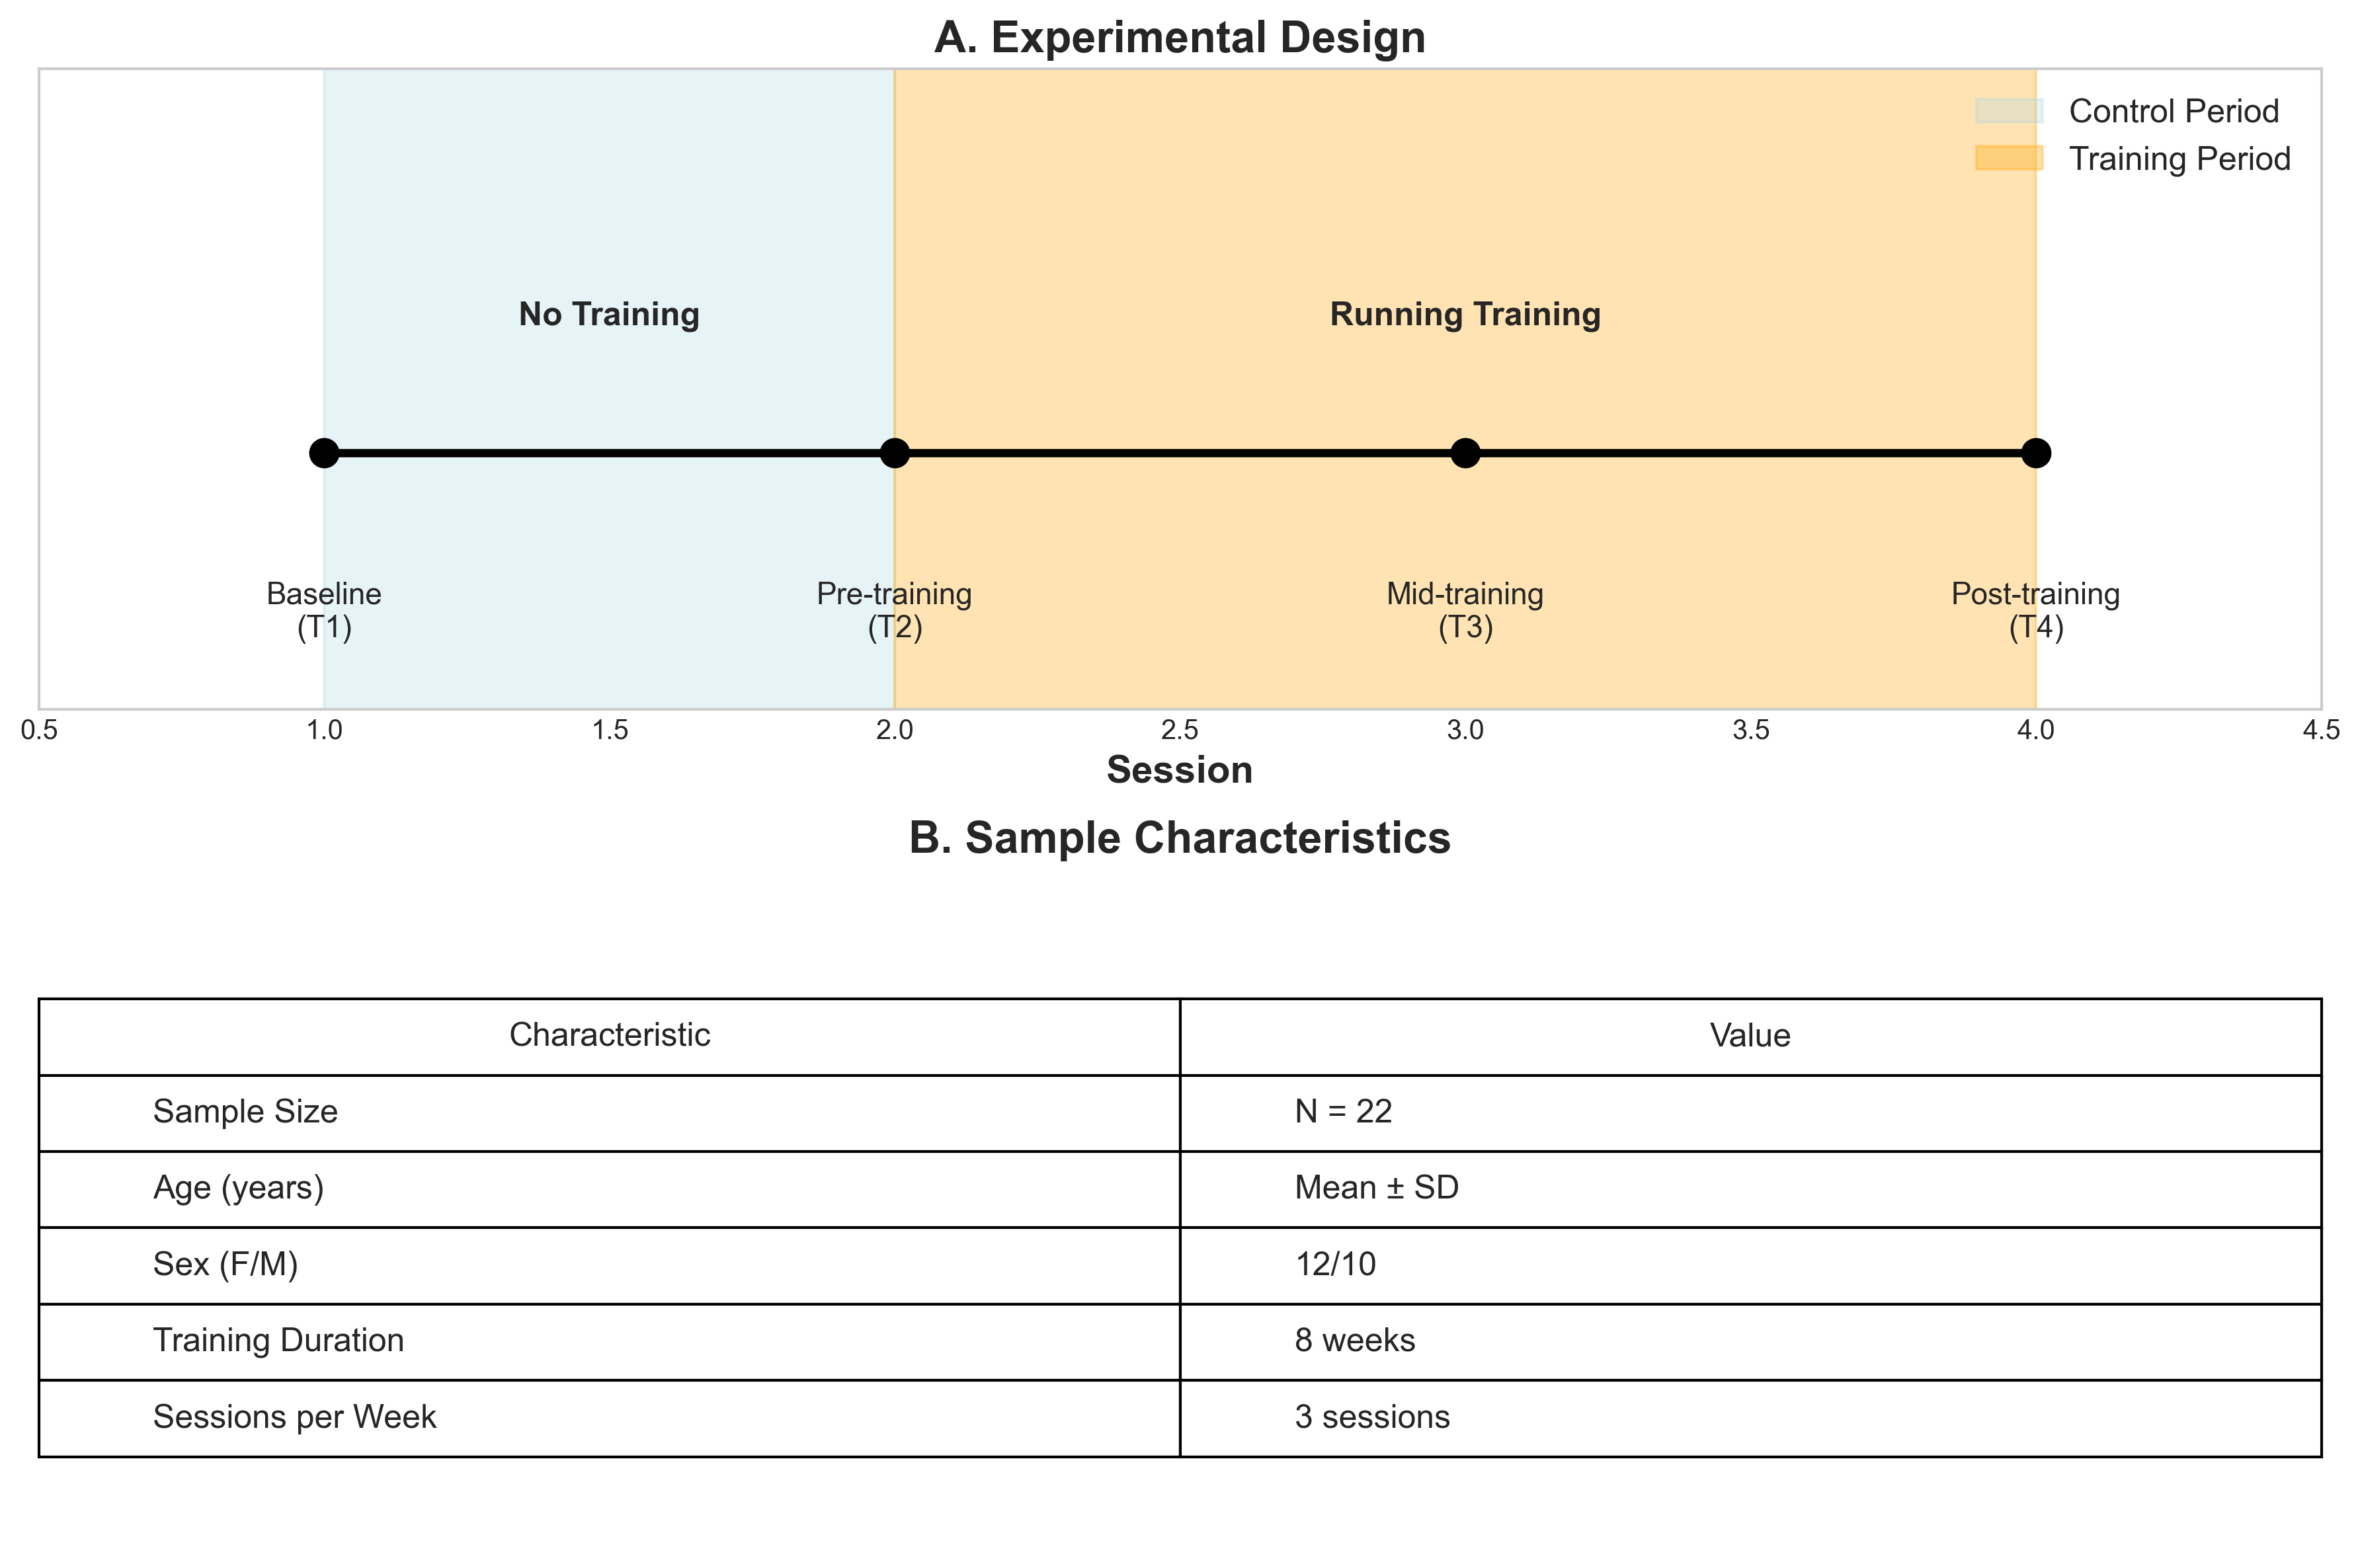
\includegraphics[width=\textwidth]{comprehensive_results/Figure1_StudyDesign.png}
\caption{\textbf{Study design and experimental timeline.} \textbf{(A)} Experimental design showing the four measurement time points: baseline (T1), pre-training (T2), mid-training (T3), and post-training (T4). The design included a 4-week control period (T1→T2) followed by an 8-week training period (T2→T4). \textbf{(B)} Sample characteristics including demographic information and training parameters.}
\label{fig:study_design}
\end{figure}

\begin{figure}[H]
\centering
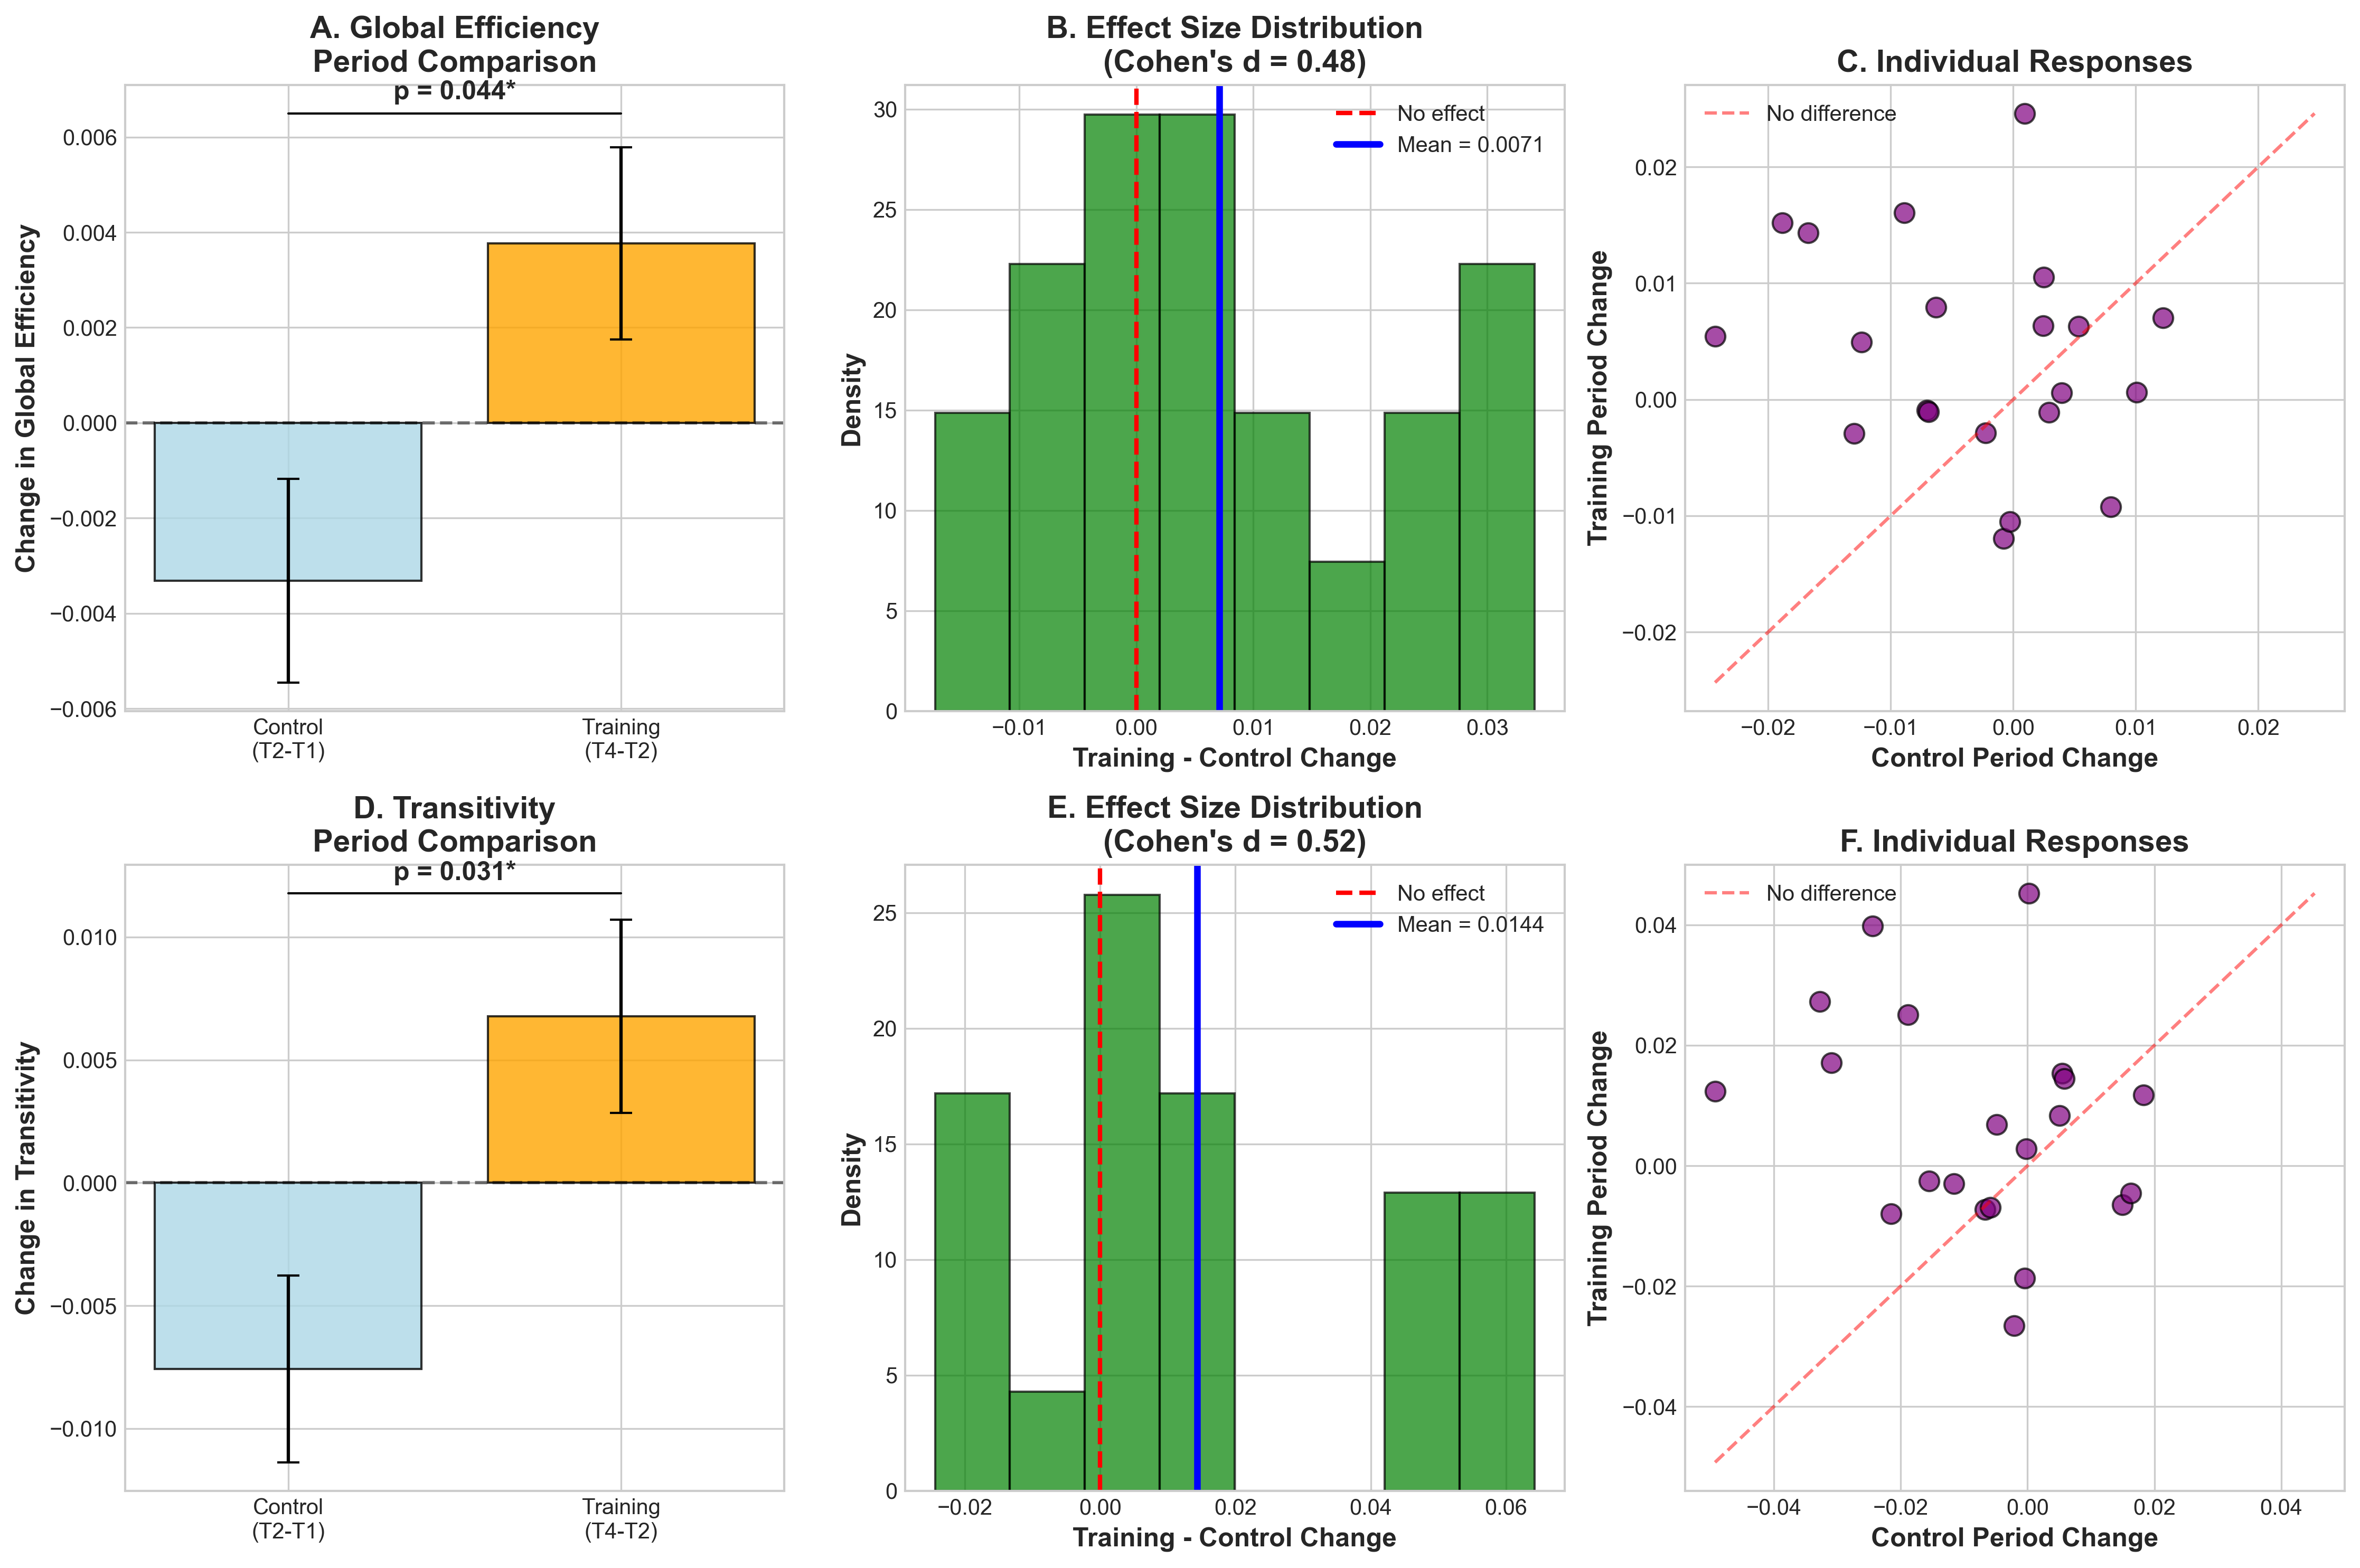
\includegraphics[width=\textwidth]{comprehensive_results/Figure2_MainResults.png}
\caption{\textbf{Training effects on global efficiency and transitivity.} \textbf{(A,D)} Period comparison showing changes during control (T2-T1) and training (T4-T2) periods. \textbf{(B,E)} Distribution of individual training effects (training change minus control change). \textbf{(C,F)} Scatter plots showing individual responses during control versus training periods. Global efficiency (A-C) showed significant training effects (p = 0.044, Cohen's d = 0.48), as did transitivity (D-F; p = 0.031, Cohen's d = 0.52). Error bars represent standard error of the mean. *p < 0.05.}
\label{fig:main_results}
\end{figure}

\begin{figure}[H]
\centering
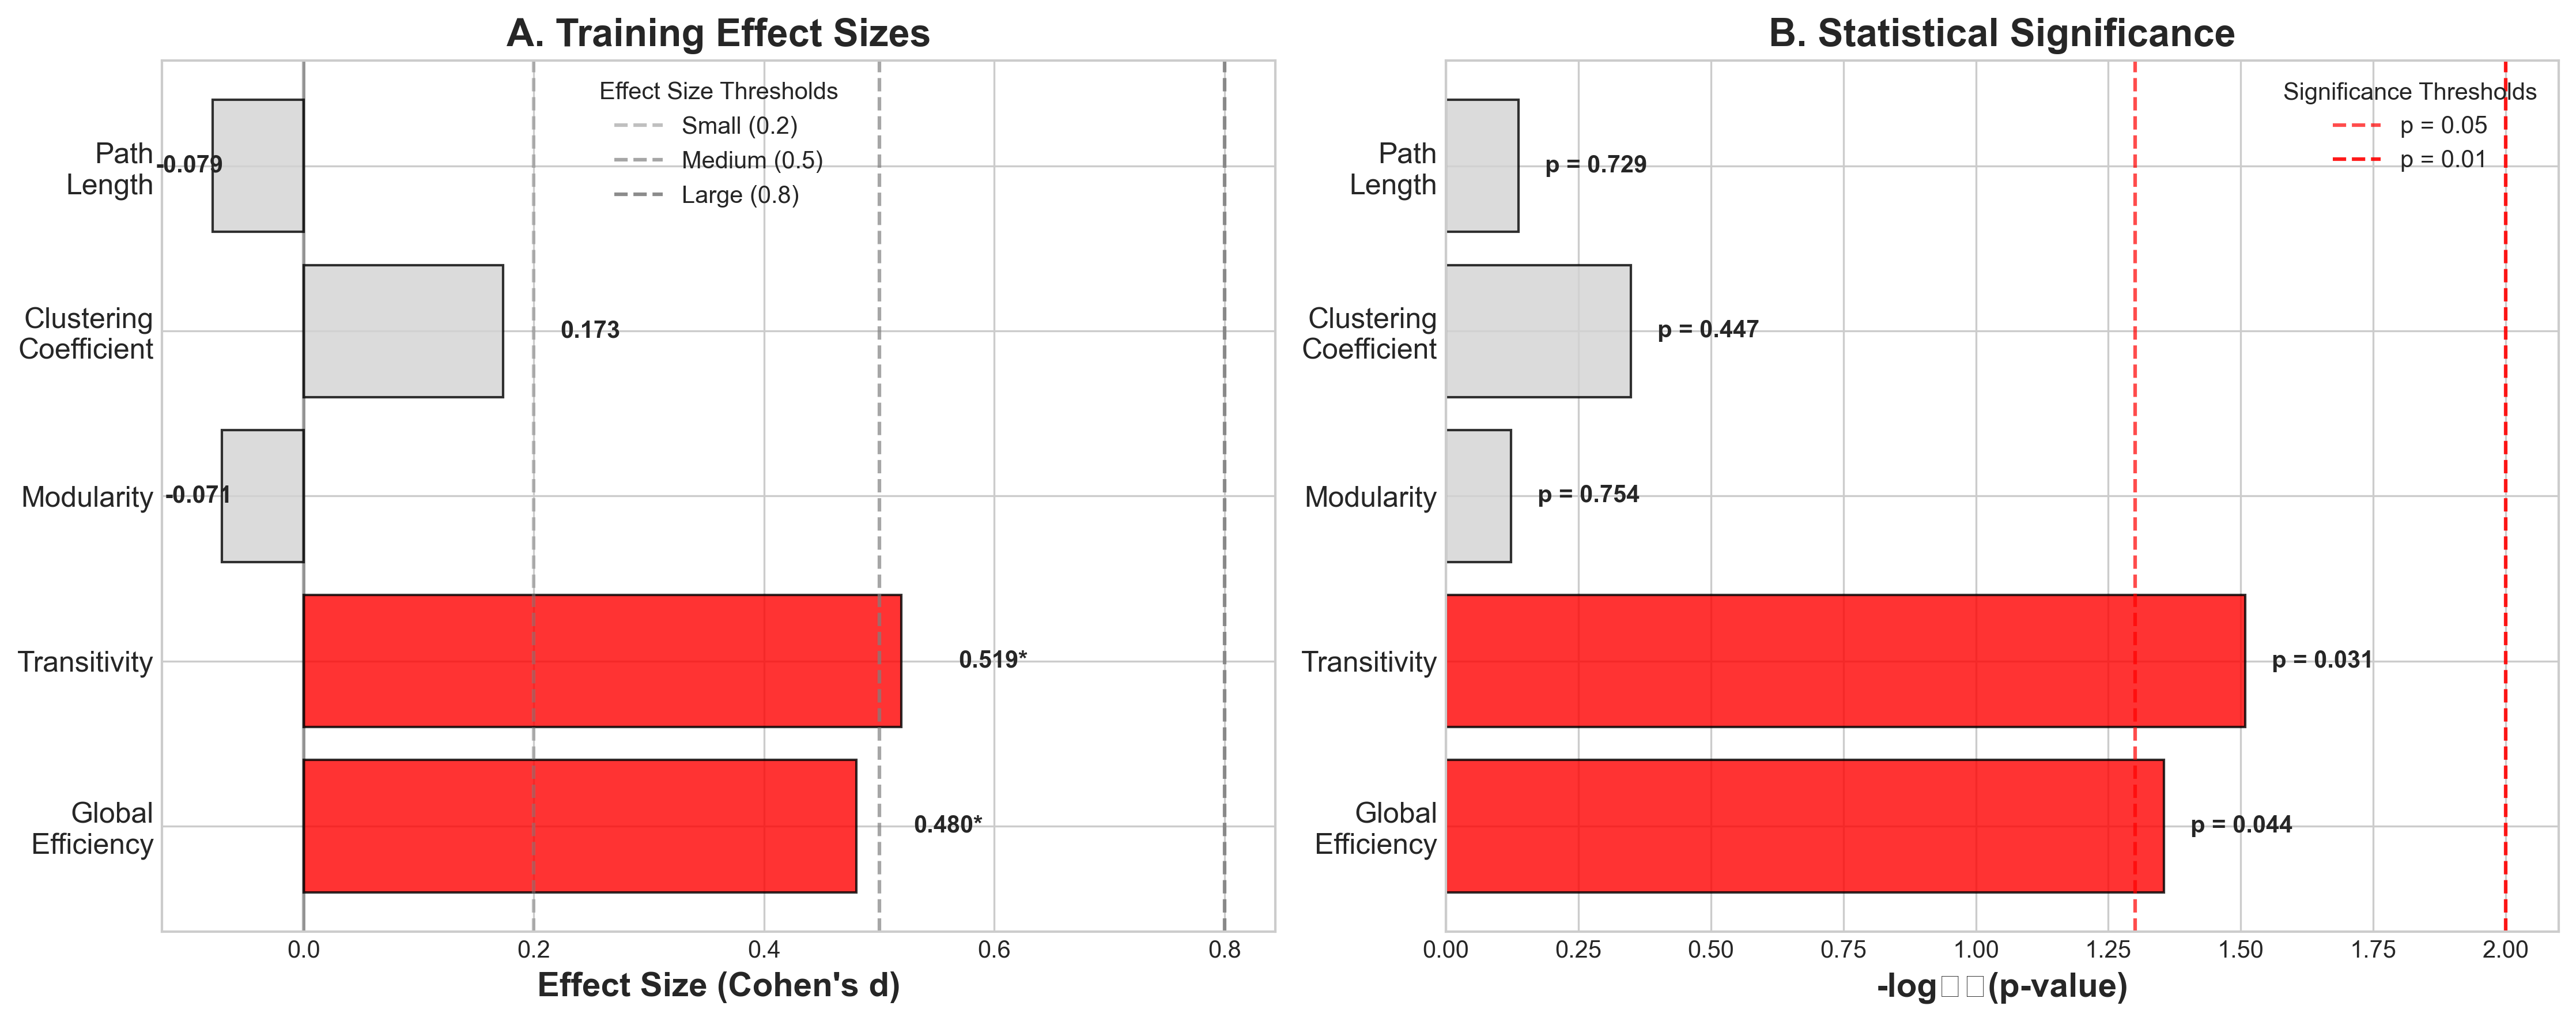
\includegraphics[width=\textwidth]{comprehensive_results/Figure3_ComprehensiveResults.png}
\caption{\textbf{Comprehensive results across all network metrics.} \textbf{(A)} Effect sizes (Cohen's d) for all analyzed metrics. Red bars indicate statistically significant effects (p < 0.05), gray bars indicate non-significant effects. Dashed lines show conventional effect size thresholds. \textbf{(B)} Statistical significance levels shown as -log₁₀(p-value). Higher values indicate greater statistical significance. Dashed lines mark p = 0.05 and p = 0.01 thresholds. Global efficiency and transitivity showed significant training effects, while modularity, clustering coefficient, and characteristic path length showed no significant changes.}
\label{fig:comprehensive_results}
\end{figure}

\newpage

% Tables
\begin{table}[H]
\centering
\caption{Descriptive statistics and training effects for all network metrics}
\label{tab:results}
\begin{tabular}{lcccccc}
\toprule
\textbf{Metric} & \textbf{Control Change} & \textbf{Training Change} & \textbf{Net Effect} & \textbf{t-statistic} & \textbf{p-value} & \textbf{Cohen's d} \\
 & \textbf{Mean ± SD} & \textbf{Mean ± SD} & \textbf{Mean ± SD} & & & \\
\midrule
Global Efficiency & 0.0027 ± 0.0189 & 0.0098 ± 0.0206 & 0.0071 ± 0.0149 & 2.17 & 0.044* & 0.48 \\
Transitivity & 0.0108 ± 0.0398 & 0.0251 ± 0.0482 & 0.0144 ± 0.0277 & 2.37 & 0.031* & 0.52 \\
Modularity & 0.0074 ± 0.0452 & 0.0058 ± 0.0449 & -0.0016 ± 0.0226 & -0.32 & 0.754 & -0.07 \\
Clustering Coefficient & 0.0001 ± 0.0007 & 0.0002 ± 0.0008 & 0.0001 ± 0.0005 & 0.78 & 0.447 & 0.17 \\
Characteristic Path Length & 0.0001 ± 0.0001 & 0.0001 ± 0.0001 & -0.0000 ± 0.0001 & -0.35 & 0.729 & -0.08 \\
\bottomrule
\end{tabular}
\\[0.5em]
\footnotesize
*p < 0.05. Control Change = T2 - T1; Training Change = T4 - T2; Net Effect = Training Change - Control Change. 
N = 21 participants with complete data. Effect sizes calculated using Cohen's d.
\end{table}

\begin{table}[H]
\centering
\caption{Post-hoc power analysis and sample size recommendations}
\label{tab:power}
\begin{tabular}{lccc}
\toprule
\textbf{Metric} & \textbf{Observed Power} & \textbf{N for 80\% Power} & \textbf{N for 90\% Power} \\
\midrule
Global Efficiency & 65\% & 35 & 47 \\
Transitivity & 72\% & 30 & 40 \\
Modularity & 8\% & 3128 & 4191 \\
Clustering Coefficient & 16\% & 271 & 362 \\
Characteristic Path Length & 8\% & 3170 & 4248 \\
\bottomrule
\end{tabular}
\\[0.5em]
\footnotesize
Power calculations based on observed effect sizes using two-tailed paired t-tests with α = 0.05.
Sample size recommendations indicate the number of participants needed to achieve specified power levels.
\end{table}

\end{document}
